\chapter{Model-based testing}
I have discovered two articles about Model-based testing, which is a Model-based testing taxonomy~\cite{Taxonomy} and an ISTQB Syllabus~\cite{Syllabus}. In this section, I want to summarize the main ideas from them.

\section{Test generation introduction}
Testing aims at showing that our implemented software and hardware system is suited for our needs. To do that, we first must specify clear goals for our testing. With testing we want to detect system failures and the differences between the expected output and the real implementation's output.

Model-based testing (MBT) is a way to clarify these differences by examine our system under test (SUT). This test approach uses a model that encodes the intended behaviour of the SUT and possibly the behaviour of its environment. This model should be simple, easy to understand according to the SUT complexity, and easy to check, modify and maintain. The model can be built in different scenarios depending on our goal of testing.

The idea of using test models is to avoid the complexity of hand-written tests, which are hard to design, maintain and write. The model can have different abstraction levels, but must contain detailed information for the automatic test generation.

MBT is basically impacts the whole test process, but does not solve everything. Any change in the requirements or in the MBT model propagates to regenerate all the tests and review the correctness, if necessary.

To fit the MBT into the developing process we must consider what inputs and outputs should be given.

Input artefacts:
\begin{itemize}
	\item Test strategy
	\item  The test basis including requirements and other test targets, test conditions, oral information and existing design or models
	\item  Incident and defect reports, test logs and test execution logs from previous test execution activities
	\item  Method and process guidelines, tool documents
\end{itemize}

Output artefacts include different kinds of test ware, such as:
\begin{itemize}
	\item  MBT models
	\item  Parts of the test plan (features to be tested, test environment), test schedule, test metrics
	\item  Test scenarios, test suites, test execution schedules, test design specifications
	\item  Test cases, test procedure specifications, test data, test scripts, test adaptation layer (specifications and code)
	\item  Bidirectional traceability matrix between generated tests and the test basis, especially requirements, and defect reports
\end{itemize}

\section{General model-based testing process}

In this section I want to describe the general process of the model-based testing in 5 steps (In figure: \figref{mbtprocess}), which was described in the article: \textit{A taxonomy of model-based testing}~\cite{Taxonomy}.

\begin{figure}[!ht]
	\centering
	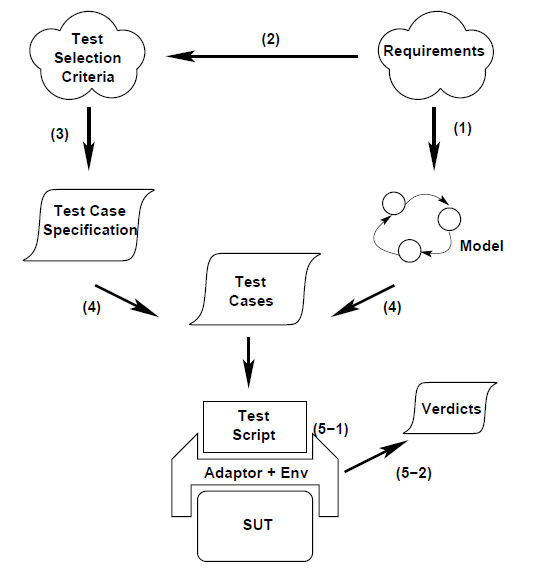
\includegraphics[width=100mm, keepaspectratio]{figures/MBTprocess.png}
	\caption{MBT process~\cite{Taxonomy}}
	\label{fig:mbtprocess} 
\end{figure}
%
\textbf{Step 1.}
Our first task is to create a model of our System Under Test (SUT), which is implemented by considering the system requirements and specification documents. Our model could have an abstract level implementation, so we can forsake some functionality or certain quality-of-service attributes.

\textbf{Step 2.}
In this step we define test selection criteria, which means that we define what is the goal of our tests. The best test is to detect all system's failures and give a helpful identifying what caused the failure. In general, test selection criteria can concentrate to functionality, structure of the model or well-defined set of faults, consequently it is a subset the model's behaviours.

\textbf{Step 3.}
The previously defined selection criteria then transformed into test case specifications. These statements formalise the notion of test selection criteria and render them operational: given a model and a test case specification, some automatic test case generator must be capable of deriving a test suite.

\textbf{Step 4.}
Test suites are generated from the model, which satisfies the test case specification (but that aggregation can be empty too). The generator pick randomly a test case from the generated set of test cases.

\textbf{Step 5-1.}
Because of the abstraction of the model, each test case input and output concretisation handled by an abstraction layer called the adaptor. The executing done by test script applying the considered input and output to the SUT. The adaptor and the script is not entirely separated from each other.

\textbf{Step 5-2.}
The adaptor (or the test script) creates a verdict, which is the result of the comparsion. This can be \textit{passed}, if the expected and the actual output conform. Otherwise the result can be \textit{failed}, which means that the expected output does not match with the actual output or \textit{inconclusive} meaning that there is no decision yet.

\section{Model-based test generation dimensions}
\paragraph{Subject of MBT models}
Basically we can set up two models for testing purposes, one for our SUT and the other for the environment of our SUT. The first one is encodes the intended behaviour of our system (as an oracle), the environment model is used to restrict the possible inputs to the SUT model (as a test selection criterion). Furthermore while creating a model consider the abstraction level of that. This can be a functional aspect (with limited functionality of the SUT), a data abstraction (expected input or/and output possibility restriction), a communication abstraction (mostly in protocol testing) and quality-of-service abstraction (like security, memory consumption).

\paragraph{Redundancy}
According to the SUT size, we can have multiple models for test suit. The models can have different aspect or different abstraction for more successful testing.

\paragraph{Quality Characteristic}
Model quality directly affects the generated test output. MBT tools may check the syntax (model is consistent with the formal rules) and at least partly, the semantic of the model (the content of the model is correct). Reviews check semantic and pragmatic quality (model is proper to test scenario and test generation).

\paragraph{Test Selection Criteria}
From the same model various test suites can be generated. Below test selection criteria will be described, which can help the tester to specify the right goal of the targeted tests. 

The coverage items may be:
\begin{itemize}
	\item \textbf{Requirements linked} to MBT model, so full requirement sheet corresponds to the test cases.
	\item \textbf{MBT model elements} set coverage items to test cases like states, transition and decision in state diagrams.
	\item \textbf{Data-related test selection criteria} is related to test design techniques and may include heuristics such as pairwise test case generation.
\end{itemize}

\paragraph{Test Generation Technology}
This have the most biggest influence to the test generation results. Test cases can be generated by random path generation algorithm, dedicated search-based algorithms, model-checking (show a counterexample), symbolic execution (to specific input, which part of the SUT executed) or deductive theorem proving (prove a statement).

\paragraph{Test execution}
MBT generated test cases can be executed by manually or automatically. For manual execution the generated tests must be usable for manual test running. For automated test execution, test cases must be generated in a form that is executable. To test the SUT from abstract tests an adaptation layer code is needed to bridge the abstraction gap. This adaptation layer can be avoided by automated test scripts.

\paragraph{On-line or Off-line test generation}
This approach is rather a technical detail of the test generation. With on-line generation, we can manipulate the SUT and test cases while executing them, which means parallel test case generation and execution. Consequently off-line generation is the idea that we create test cases before they are run.

\section{Model-based test generation tools}
In this section I want to describe the Graphwalker (\ref{mbt:tools:graphwalker}) and the Spec Explorer tool (\ref{mbt:tools:specExplorer}), which I have discovered in this semester.

\subsection{Graphwalker} \label{mbt:tools:graphwalker}

GraphWalker is an open source model-based testing tool for MBT. It is designed to make directed graph based models easily for testing purposes. The given graphs can be connected to each other, and can have variables too. The tool generates test paths from these given graphs. Each graph will have it's own set of generator(s) and stop condition(s). An edge in the directed graph represent an action in the system, consequently a vertex means a verification state, where we can have assertions in code. A path is used to call the corresponding methods or functions of our SUT (system under test) by the adapter layer. 

The test selection is implemented by an expression, which have the following template: generator(stop\_condition\_type(condition))). This describes how to cover (random, a\_star, shortest\_all\_paths) and what to cover (requirement, edge, vertex, time and their variations).

There are two ways to generate tests by GraphWalker:
\begin{itemize}
	\item Offline: The path generation from the graph is done once (typically with command line), and these tests needs to be stored. A test automation system handle the tests. 
	\item Online: The path generation from the graph is created during the execution of the tests, run-time. If you have java coded SUT, it is pretty easy to add annotations to SUT and connect that to the generated paths. (command for Maven: \textit{mvn graphwalker:test})
\end{itemize}

For test execution an interface from the models is created by \textit{graphwalker:generate-sources} command. Our job is to implement these interfaces and call the proper SUT functionality for the given edges and vertexes.

\subsection{Spec Explorer} \label{mbt:tools:specExplorer}

It is a tool that extends  Microsoft Visual Studio for creating models of software behaviour, analysing those models with graphical visualization, checking the validity of those models, and generating test cases from the models. The environment incorporate into our solution in Visual Studio, with a project, that contains a model (adapts the test generation script to the implementation), and a cord file (sets up the SpecExplorer settings). We can create several instances from the model and cord file in the same project.

The complex SpecExplorer environment gives us validation, exploration and test generation opportunities through developing/testing our system. Validation check the consistency of the cord and model programs, then exploration can give graph represented behaviour description about the SUT. In the last steps we can generate test code from the selected machines, which results in standalone unit test cases, which can be run by the other Visual Studio tools. Important information about the selected machines, that these must have TestEnabled and ForExploration flags in the cord files.


